% Carried over verbatim from monograph/main.tex (Study 1 record, 13 Sep 2026).
\chapter{Motivation and problem formulation}\label{s1:ch:ch02_motivation_and_problem_formulation}

\section{Why cervical cytology makes independence important}

Cervical cancer caused an estimated 660,000 new cases and 350,000 deaths worldwide in 2022~\cite{who2025hpv}. Cytology screening is a high-volume recognition problem: a small number of clinically important abnormal cells must be found among many plausible normal cells. Automation is attractive because it can help direct expert attention, but only if reported generalization represents genuinely unseen biological or acquisition units.

Modern cervical-cell classifiers report very high crop-level scores. DeepPap reported 98.3\% on Herlev~\cite{zhang2017deeppap}; DeepCervix reported 99.14\% on SIPaKMeD~\cite{rahaman2021deepcervix}; and a knowledge-distillation system reported 98.52\% on SIPaKMeD~\cite{gao2022knowledge}. These achievements motivated a basic audit question that is logically prior to choosing a stronger network: \emph{what population unit does the test set represent?}

\section{Observation, parent, and evaluation unit}

Let $x_i$ be a released image observation and let $g(x_i)=p_j$ map it to the acquisition unit that generated it. In this project:
\begin{itemize}
  \item $x_i$ is a SIPaKMeD cell crop and $p_j$ is a cluster field;
  \item $x_i$ is a Cx22 generated region and $p_j$ is a CCEDD source image;
  \item $x_i$ is a CRIC annotated cell and $p_j$ is its source smear image;
  \item $x_i$ is a Herlev single-cell image and is also its own parent.
\end{itemize}

The crucial idea is that the \emph{model input} and the \emph{independent sampling unit} need not be the same object. A network consumes $x_i$, but the statistical independence boundary may be $p_j$.

\begin{figure}[H]
\centering
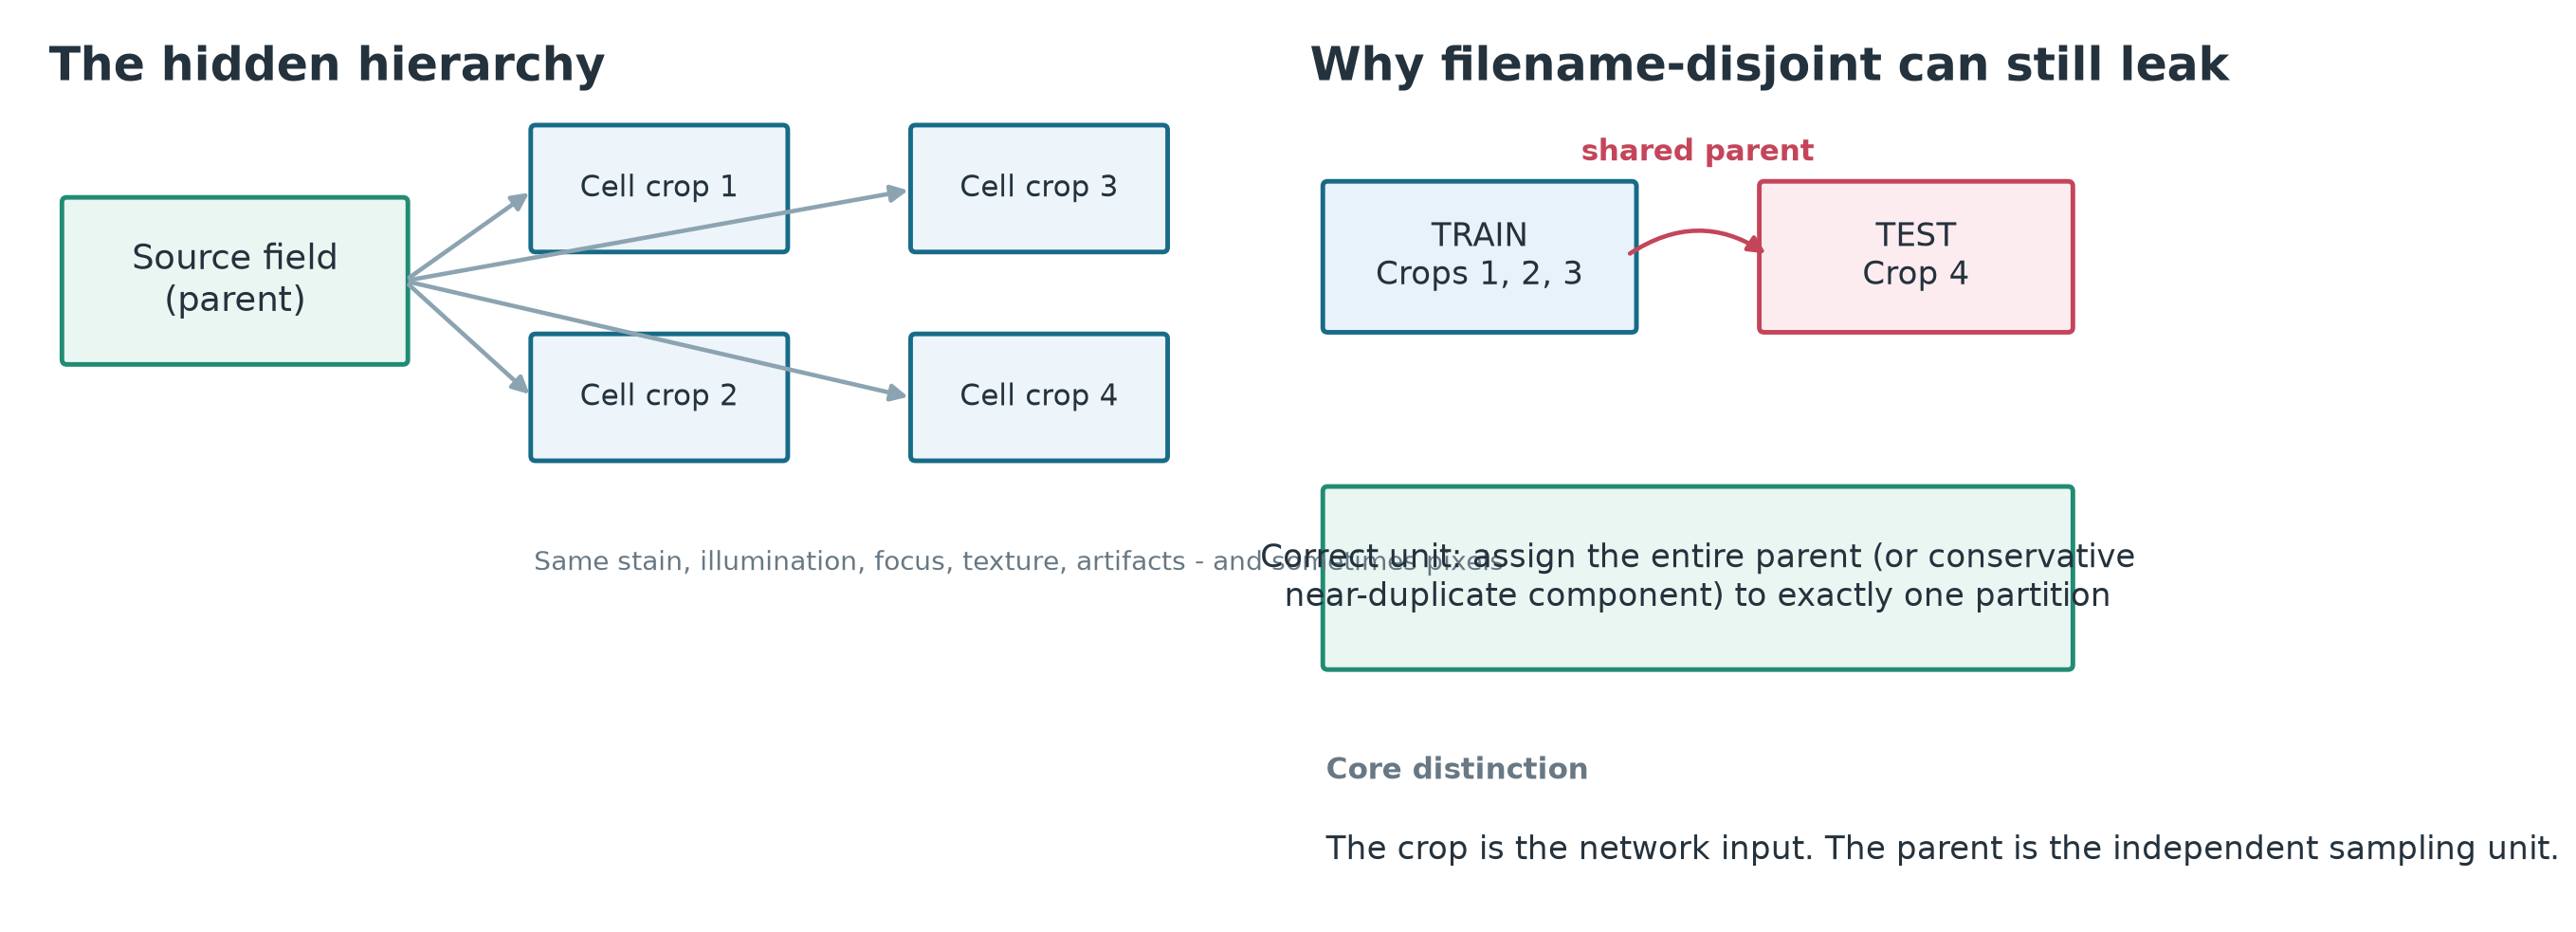
\includegraphics[width=\textwidth]{hierarchy_and_leakage.png}
\caption{The hidden hierarchy and the central failure mode. Several file-disjoint crops can share a parent field, source-specific nuisance factors, or literal source pixels.}
\label{s1:fig:hierarchy}
\end{figure}

\section{Three different claims that must not be conflated}

\begin{keybox}{Claim 1: structural non-independence}
Some parents contribute observations to both train and test. This can be established exactly from provenance and split assignments. It requires no model.
\end{keybox}

\begin{keybox}{Claim 2: shortcut availability}
A model can identify the source parent from held-out sibling crops at greater-than-chance accuracy. This shows that parent information survives in the released input. It does not yet show that a disease or morphology classifier uses it.
\end{keybox}

\begin{keybox}{Claim 3: downstream score inflation}
A crop-level protocol produces a larger score than a parent-disjoint protocol under matched models, seeds, and sample sizes. This is an empirical paired comparison. It needs uncertainty, multiplicity correction, and careful interpretation.
\end{keybox}

The project obtains strong evidence for Claims 1 and 2. For Claim 3, point estimates are directionally consistent across every tested architecture, but the confirmatory families do not cross the multiplicity-adjusted threshold. The report therefore never upgrades ``available shortcut'' into ``proven universal causal inflation.''

\section{Relationship to leakage and duplicate audits}

Duplicate-aware evaluation has been studied in general vision: ciFAIR removed near-duplicate CIFAR test counterparts~\cite{barz2020cifair}; license-plate work re-evaluated models under duplicate-free splits~\cite{laroca2023lpr}; and medical-image re-identification demonstrated that patient identity can be highly learnable~\cite{packhauser2022reidentification}. Kapoor and Narayanan place these problems in a broader taxonomy of data leakage and reproducibility failures~\cite{kapoor2023leakage}. CytoFair's distinctive concern is an exact cervical-cytology source hierarchy: sibling crops can be non-independent without being duplicate files.
